\documentclass{article}
% Language setting
% Replace `english' with e.g. `spanish' to change the document language
\usepackage[english]{babel}


% Set page size and margins
% Replace `letterpaper' with `a4paper' for UK/EU standard size
\usepackage[a4paper,top=2cm,bottom=2cm,left=3cm,right=3cm,marginparwidth=1.75cm]{geometry}

% Useful packages
\usepackage[utf8]{inputenc}
\usepackage{fontspec} 
\setmonofont{Fira Code}[Scale=0.9]

\usepackage{array}
\usepackage[most]{tcolorbox} % for inline code
\usepackage{amsmath}
\usepackage{graphicx}
\usepackage{subfigure}
\usepackage[colorlinks=true, allcolors=blue]{hyperref}
\usepackage{authblk}
\usepackage{amssymb}
\usepackage{listings}
\usepackage{color}
\usepackage{xcolor}
\usepackage{float}
\usepackage{biblatex} %Imports biblatex package
\addbibresource{references.bib} %Import the bibliography file
\usepackage{wrapfig}
\usepackage{booktabs}
\usepackage{longtable}

\renewcommand{\floatpagefraction}{0.1}
\renewcommand{\textfraction}{0}

\definecolor{dkgreen}{rgb}{0,0.6,0}
\definecolor{gray}{rgb}{0.5,0.5,0.5}
\definecolor{mauve}{rgb}{0.58,0,0.82}
\definecolor{lightgray}{gray}{0.9}

\lstdefinestyle{pythonstyle}{
  language=Python,
  frame=tb,
  aboveskip=3mm,
  belowskip=3mm,
  showstringspaces=false,
  columns=flexible,
  basicstyle={\ttfamily\small},
  numbers=left,
  numberstyle=\tiny\color{gray},
  keywordstyle=\color{blue},
  commentstyle=\color{green!50!black},
  stringstyle=\color{red!70!black},
  breaklines=true,
  breakatwhitespace=true,
  tabsize=4,
  captionpos=b,
  morekeywords={self, cls, __init__, None},
}

\lstdefinestyle{pseudocode}{frame=tb,
  language=Python,
  aboveskip=3mm,
  belowskip=3mm,
  showstringspaces=false,
  columns=flexible,
  basicstyle={\small\ttfamily},
  numbers=left,
  numberstyle=\tiny\color{gray},
  keywordstyle=\color{blue},
  commentstyle=\color{dkgreen},
  stringstyle=\color{mauve},
  breaklines=true,
  breakatwhitespace=true,
  tabsize=3
}

\lstdefinestyle{input}{frame=none,
  aboveskip=3mm,
  belowskip=3mm,
  showstringspaces=false,
  columns=flexible,
  basicstyle={\small\ttfamily},
  numbers=none,
  numberstyle=\tiny\color{gray},
  keywordstyle=\color{blue},
  commentstyle=\color{dkgreen},
  stringstyle=\color{mauve},
  breaklines=true,
  breakatwhitespace=true,
  tabsize=3,
  captionpos=b,
}

% inline code display
\newtcbox{\inlinecode}{
  nobeforeafter, 
  colback=lightgray, 
  colframe=white, 
  boxrule=0pt, 
  arc=1mm, 
  left=0pt, right=0pt, top=0pt, bottom=0pt,
  on line,
  fontupper=\scriptsize\ttfamily
}


% make title
\title{
\includegraphics[scale=0.2]{Cam_logo_bw.png}\\
\vspace{0.5cm}
S1 Statistical Methods Coursework
}
\author{xl628}
\affil{Department of Physics, University of Cambridge}

\begin{document}

\maketitle

\vspace{1cm}
\noindent
\textbf{Document Statistics:} \\
Words in text: 1590 \\
Words in headers: 79 \\
Words outside text (captions, etc.): 178 \\
Number of headers: 25 \\
Number of floats/tables/figures: 8 \\
Number of math inlines: 116 \\
Number of math displayed: 20

\section{Crystal Ball Normalization}

The Crystal Ball probability distribution is defined as:

$$
p(X; \mu, \sigma, \beta, m) = N \cdot
\begin{cases}
e^{-Z^2/2}, & \text{for } Z > -\beta \\
\left(\frac{m}{\beta}\right)^m e^{-\beta^2/2} \left(\frac{m}{\beta} - \beta - Z\right)^{-m}, & \text{for } Z \leq -\beta
\end{cases}
$$

where \( Z = \frac{X - \mu}{\sigma} \) is the standard normal transformation for a random variable $X$ at location, $\mu$, with scale, $\sigma$. The distribution is only valid when \( \beta > 0 \) and \( m > 1 \).

\paragraph{Proof}

By definition, the normalization requires:

$$
\int_{-\infty}^{\infty} p(X; \mu, \sigma, \beta, m)\, dX = 1.
$$

Rewrite the normalization in terms of $Z$. Since $ dX = \sigma\, dZ $:

$$
1 = \int_{-\infty}^{\infty} N \cdot p_z(Z) \sigma\, dZ,
$$

This gives:

\begin{equation}
\label{eq:I1I2}
    1 = N \sigma \left[ \int_{-\infty}^{- \beta} \left(\frac{m}{\beta}\right)^m e^{-\beta^2/2} \left(\frac{m}{\beta} - \beta - Z\right)^{-m} dZ \;+\; \int_{-\beta}^{\infty} e^{-Z^2/2} dZ \right] = N \sigma(I_1 + I_2).
\end{equation}



Consider the integral:

$$
I_1 = \int_{-\infty}^{- \beta} \left(\frac{m}{\beta}\right)^m e^{-\beta^2/2} \left(\frac{m}{\beta} - \beta - Z\right)^{-m} dZ.
$$

Factor out the constants:

\begin{equation}
\label{eq:I1}
    I_1 = \left(\frac{m}{\beta}\right)^m e^{-\beta^2/2} \int_{-\infty}^{- \beta} \left(\frac{m}{\beta} - \beta - Z\right)^{-m} dZ.
\end{equation}

Use the substitution:

$$
t = \frac{m}{\beta} - \beta - Z \implies dZ = -dt.
$$

When $ Z = -\infty $, we have $ t \to \infty $.  
When $ Z = -\beta $, we get $t = \frac{m}{\beta} - \beta - (-\beta) = \frac{m}{\beta}.$

So the integral limits transform as $ Z: -\infty \to -\beta $ to $ t: \infty \to \frac{m}{\beta} $:

$$
I_1 = \left(\frac{m}{\beta}\right)^m e^{-\beta^2/2} \int_{\infty}^{m/\beta} t^{-m}(-dt) = \left(\frac{m}{\beta}\right)^m e^{-\beta^2/2} \int_{m/\beta}^{\infty} t^{-m} dt.
$$

The integral $\int t^{-m} dt = \frac{t^{-m+1}}{-m+1}$ for $m > 1$. Thus:

$$
I_1 = \left(\frac{m}{\beta}\right)^m e^{-\beta^2/2} \left(\frac{(m/\beta)^{-m+1}}{m-1} \right) = e^{-\beta^2/2} \frac{m}{\beta(m-1)}.
$$

Now consider the second integral:

\begin{equation}
\label{eq:I2}
    I_2 = \int_{-\beta}^{\infty} e^{-Z^2/2} dZ.
\end{equation}

This integral can be expressed in terms of the standard normal CDF $\Phi(z)$, where

$$
\Phi(z) = \frac{1}{\sqrt{2\pi}} \int_{-\infty}^{z} e^{-t^2/2} dt.
$$

We note:
$$
\int_{-\beta}^{\infty} e^{-Z^2/2} dZ = \sqrt{2\pi}\big[ \Phi(\infty) - \Phi(-\beta) \big] = \sqrt{2\pi}\left[1 - \Phi(-\beta)\right].
$$

Therefore:

$$
I_2 = \sqrt{2\pi} \left[ 1 - \Phi(-\beta) \right] = \sqrt{2\pi} \Phi(\beta).
$$

Substituting $I_1$ (Eq. \ref{eq:I1}) and $I_2$ (Eq. \ref{eq:I2}) back into Eq. \ref{eq:I1I2}, we have:

$$
1 = N \sigma [I_1 + I_2] = N \sigma \left[ \frac{m}{\beta(m-1)} e^{-\beta^2/2} + \sqrt{2\pi} \,\Phi(\beta) \right].
$$

Thus, we have proven that:

$$
N^{-1} = \sigma \left[ \frac{m}{\beta(m - 1)} e^{-\beta^2/2} + \sqrt{2\pi}\,\Phi(\beta) \right].
$$

\section{Module Development}

Several classes implementing the required distributions are provided in \texttt{src/pdfs\_numba\_stats.py}. 

Throughout the project, the computational efficiency of probability density functions (PDFs) and cumulative distribution functions (CDFs) has been a critical factor, significantly influencing the speed of sample generation and optimization. Various measures have been implemented to enhance this efficiency:

\paragraph{Library Choice} 
We employ \inlinecode{numba-stats}\cite{hans_dembinski_2024_13236518} instead of \inlinecode{scipy.stats} due to its substantial performance improvements. It enables faster computations, conveniently supports direct operations on NumPy arrays, and eliminates the need for manual function vectorization.

\paragraph{Class-Based Programming}
Class-based programming is utilized throughout the development process. Parameters and methods specific to each distribution, such as \inlinecode{pdf}, \inlinecode{cdf}, and their truncated versions, are encapsulated within the classes.

Class initialization allows for one-time parameter passing and pre-computation of values, such as normalization constants for truncated functions. This approach reduces redundant calculations during method calls, leading to significant performance improvements.


\subsection{Normalization Test}

To ensure the accuracy of the defined distributions, we verified their normalization numerically in \texttt{notebooks/b\_c\_norm\_visualization.ipynb}.

The signal-background model is defined as follows:

$$
f(X, Y) = f g_s(X)h_s(Y) + (1 - f)g_b(X)h_b(Y).
$$

Using \inlinecode{integrate.quad} and \inlinecode{integrate.dblquad}, we validated the normalization of the following components:
\begin{itemize}
    \item $g_s(X)$ over $X \in [0, 5]$,
    \item $g_b(X)$ over $X \in [0, 5]$,
    \item $h_s(Y)$ over $Y \in [0, 10]$,
    \item $h_b(Y)$ over $Y \in [0, 10]$,
    \item $s(X, Y) = g_s(X)h_s(Y)$ over $X \in [0, 5]$ and $Y \in [0, 10]$,
    \item $b(X, Y) = g_b(X)h_b(Y)$ over $X \in [0, 5]$ and $Y \in [0, 10]$,
    \item $f(X, Y) = f g_s(X)h_s(Y) + (1 - f)g_b(X)h_b(Y)$ over $X \in [0, 5]$ and $Y \in [0, 10]$,
\end{itemize}

The parameters used are:
\begin{lstlisting}[style=pythonstyle]
signal_params = {
    'mu': 3, 
    'sigma': 0.3, 
    'beta': 1, 
    'm': 1.4, 
    'decay_rate': 0.3
}
background_params = {
    'mu_bg': 0, 
    'sigma_bg': 2.5
}

f = 0.6  # Signal fraction
x_min, x_max = 0, 5
y_min, y_max = 0, 10
\end{lstlisting}

The following output confirms proper normalization of the distributions:
\begin{lstlisting}[style=input]
1D Normalizations:
- Signal X distribution          1.000
- Background X distribution      1.000
- Signal Y distribution          1.000
- Background Y distribution      1.000

2D Normalizations:
- Total distribution             1.000
- Signal XY distribution         1.000
- Background XY distribution     1.000
\end{lstlisting}


\section{Distribution Visualization}

For the signal-background model:
$$
f(X, Y) = f g_s(X)h_s(Y) + (1 - f)g_b(X)h_b(Y),
$$
we can integrate out $X$ or $Y$ to obtain marginal distributions. Given the separability of $X$ and $Y$ and the rectangular integration range, the one-dimensional projections are:
$$
g(X) = \int f(X,Y) dY = f g_s(X) + (1 - f) g_b(X),
$$
$$
h(Y) = \int f(X,Y) dX = f h_s(Y) + (1 - f) h_b(Y).
$$


Thus, we can plot the one-dimensional projections of these distributions in both the variables $X$ and $Y$ in Fig. \ref{fig:two_dists} and the joint distribution in Fig. \ref{fig:joint}.

\begin{figure}[!h]
    \centering
    \subfigure[]{
        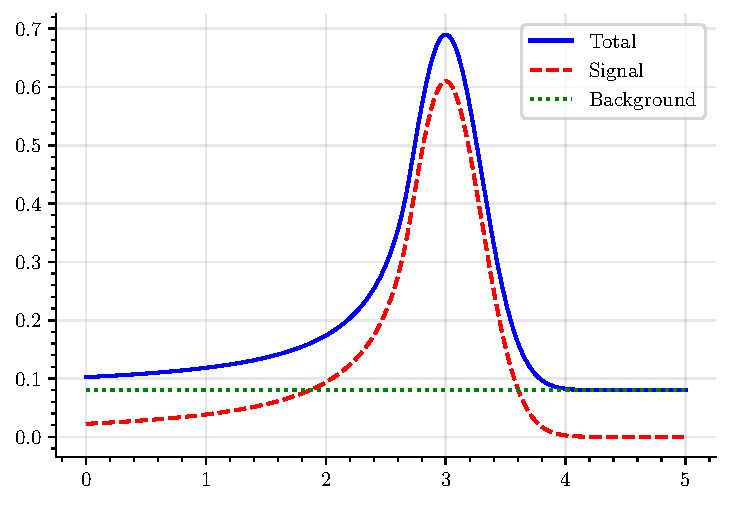
\includegraphics[width=0.47\textwidth]{./images/marginal_x.pdf}
        \label{fig:dist-1}
    }
    \hspace{0.0\textwidth}
    \subfigure[]{
        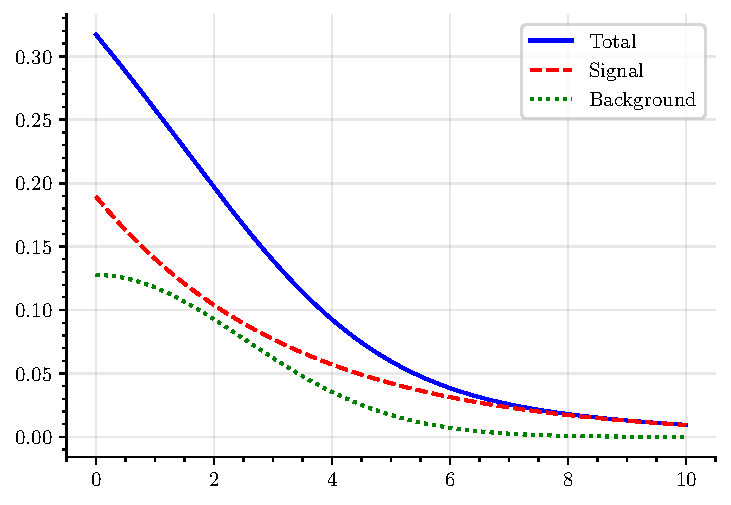
\includegraphics[width=0.47\textwidth]{./images/marginal_y.pdf}
        \label{fig:dist-2}
    }
    \caption{(a) Probability density function $g(X) = f g_s(X) + (1-f) g_b(X)$, signal component $f g_s(X)$, and background component $(1-f) g_b(X)$ (marginal distributions in $X$). 
    (b) Probability density function $h(Y) = f h_s(Y) + (1-f) h_b(Y)$, signal component $f h_s(Y)$, and background component $(1-f) h_b(Y)$ (marginal distributions in $Y$).}
    \label{fig:two_dists}
\end{figure}


\begin{figure}[!htbp]
\centering
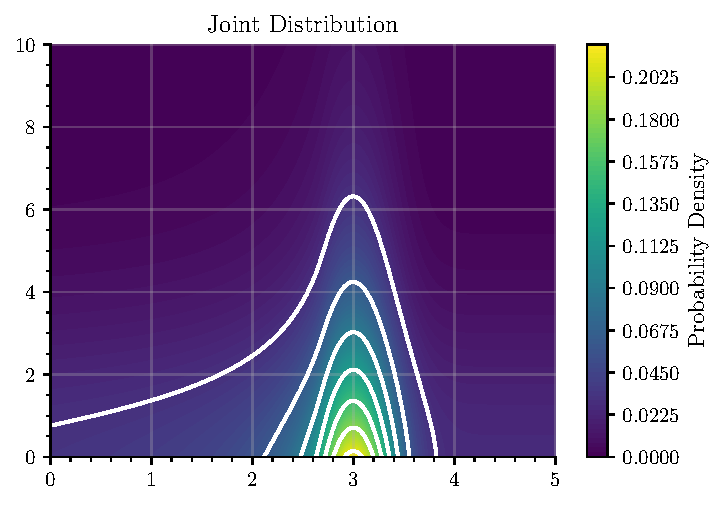
\includegraphics[width=0.47\textwidth]{./images/joint_distribution.pdf}
\caption{Two-dimensional plot of the joint probability density.}
\label{fig:joint}
\end{figure}


\section{Sampling and Fitting}

\begin{figure}[!htbp]
\centering
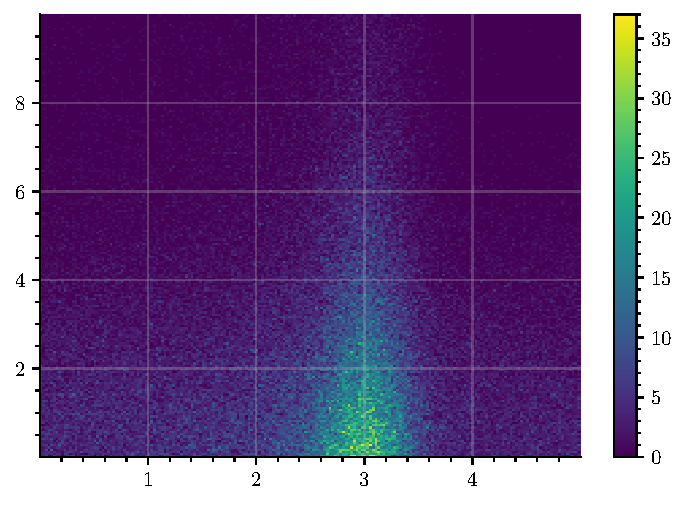
\includegraphics[width=0.47\textwidth]{./images/accept_reject_sampling.pdf}
\caption{Data generated using the Accept-Reject Method.}
\label{fig:gd}
\end{figure}

\subsection{Accept-Reject Method}

Since the percentage point function (PPF) is not easily obtainable in this case, we implement the accept-reject method to generate samples from the model.

The maximum of the probability density function (PDF) can sometimes be derived analytically. Because $X$ and $Y$ are separable, and with respect to $X$, both the signal and background (uniform) components achieve their maximum at the same $X$ value. When $\mu_b = 0$, the signal and background components with respect to $Y$ reach their maximum at $Y = 0$.

For the given parameters where $\mu_b = 0$, the analytical maximum occurs at $(3.0, 0.0)$.

The implementation is detailed in the function \inlinecode{accept\_reject\_sampling\_2d} from \texttt{notebooks/d} \texttt{\_gen\_sample\_estimate.ipynb}. To accelerate the process, candidate points are generated in batches, leveraging vectorized computations for efficiency.

The generated data is stored in \texttt{notebooks/samples.npy}, and the corresponding visualization is shown in Fig. \ref{fig:gd}.



\subsection{Extended Maximum Likelihood Estimate (EMLE)}

We implemented both unbinned and binned fits in \texttt{notebooks/d\_gen\_sample\_estimate.ipynb} using the \inlinecode{iminuit} library\cite{iminuit}. 

For consistency, the same starting point and 29 bins were used for the binned fit. The parameter estimates and their estimated uncertainties (Hesse errors) from one run are presented in Table \ref{tab:fit}.

\begin{longtable}{lll}
\caption{Comparison of unbinned and binned EMLE with estimated values and Hesse errors.} \label{tab:fit}\\
\toprule
\textbf{Name} & \textbf{Value} & \textbf{Hesse Error} \\
\midrule
\multicolumn{3}{l}{\textbf{Unbinned EMLE}} \\
$N$ & $100.00\times10^3$ & $0.32\times10^3$ \\
$\mu$ & 2.9986 & 0.0028 \\
$\sigma$ & 0.3022 & 0.0026 \\
$\beta$ & 0.969 & 0.025 \\
$m$ & 1.45 & 0.07 \\
$\lambda$ & 0.3010 & 0.0021 \\
$\mu_{bg}$ & 0.04 & 0.08 \\
$\sigma_{bg}$ & 2.46 & 0.04 \\
$f$ & 0.601 & 0.004 \\
\midrule
\multicolumn{3}{l}{\textbf{Binned EMLE}} \\
$N$ & $100.00\times10^3$ & $0.32\times10^3$ \\
$\mu$ & 2.9974 & 0.0028 \\
$\sigma$ & 0.3031 & 0.0027 \\
$\beta$ & 0.981 & 0.025 \\
$m$ & 1.42 & 0.07 \\
$\lambda$ & 0.3012 & 0.0021 \\
$\mu_{bg}$ & 0.05 & 0.08 \\
$\sigma_{bg}$ & 2.46 & 0.04 \\
$f$ & 0.602 & 0.004 \\
\bottomrule
\end{longtable}

A visualization of the unbinned EMLE estimate for parameter $N$ is shown in Fig. \ref{fig:profile_N}.

\begin{figure}[!t]
\centering
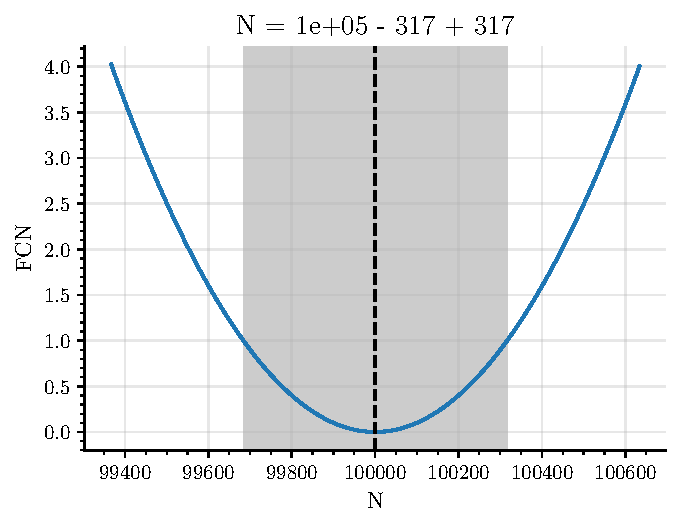
\includegraphics[width=0.47\textwidth]{./images/profile/N_profile.pdf}
\caption{Estimate of $N$ and its uncertainty.}
\label{fig:profile_N}
\end{figure}


The binned fit is significantly faster than the unbinned fit while maintaining comparable accuracy. Additionally, the execution time for sampling and binned fitting was evaluated using the \inlinecode{\%timeit} command:

\begin{lstlisting}[style=pythonstyle]
%timeit -n 100 np.random.normal(size=100000) # benchmark
%timeit -n 100 accept_reject_sampling_2d(model.pdf, 100000, x_min, x_max, y_min, y_max, f_max_3)
%timeit -n 100 optimize_binned()
\end{lstlisting}

The measured execution times were as follows:

\begin{lstlisting}[style=input]
2.91 ms ± 770 μs per loop (mean ± std. dev. of 7 runs, 100 loops each)
79.1 ms ± 1.43 ms per loop (mean ± std. dev. of 7 runs, 100 loops each)
54.6 ms ± 1.23 ms per loop (mean ± std. dev. of 7 runs, 100 loops each)
\end{lstlisting}


\section{Multi-Dimensional Fit and Parametric Bootstrap}
\label{sec:pbe}

In this section, we employ a multi-dimensional likelihood estimate to fit the signal-background model and implement parametric bootstrapping to assess the robustness of this procedure.


\paragraph{Generating Real Data}
We continue using the accept-reject sampling method to generate data, but introducing a Poisson variation in the sample size. This is implemented in the function \inlinecode{accept\_reject\_sampling\_2d\_with\_Poisson} in \texttt{notebooks/e\_bootstrapping.ipynb}.



\paragraph{Fitting the Data}
The data is fitted using the unbinned Extended Maximum Likelihood Estimation (EMLE) method to determine the "true" parameters for bootstrapping. Given that the sample sizes in this task are relatively small, the unbinned method is preferred over the binned method.

\paragraph{Bootstrap Procedure}
We use the \inlinecode{bootstrap} function from the \inlinecode{resample} package\cite{scikit-hep_resample} to generate an ensemble of 250 samples for the bootstrapping process.

\begin{lstlisting}[style=pythonstyle]
boot_samples = np.array( [ b for b in bootstrap.resample(samples, size=250) ] )
\end{lstlisting}

\paragraph{Fitting the Bootstrap Ensemble}
To check for any bias in the estimation method, we fit the generated samples back into the model and evaluate their deviation from the "true" value. Specifically, we analyze the parameter $\lambda$.

For real data generated with $N = 1000$ (with actual Poisson-adjusted sample size of 988), we fit the pseudo-experiments and get the expectation of the estimate and the uncertainty of the estimate, the expectation of the estimated uncertainty (Hesse error) and uncertainty of it in Fig. \ref{fig:samplingest_1000}. 

\begin{figure}[!htbp]
\centering
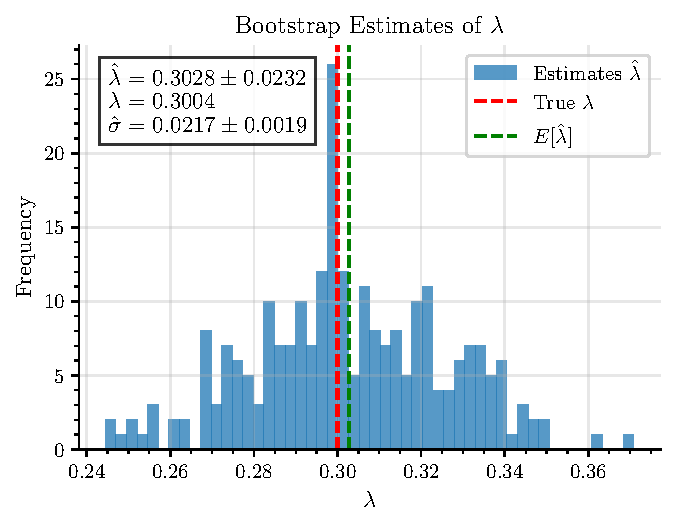
\includegraphics[width=0.47\textwidth]{./images/bootstrap_estimates.pdf}
\caption{Bootstrap estimates of $\lambda$ for a sample size of 1000.}
\label{fig:samplingest_1000}
\end{figure}

\paragraph{Impact of Sample Size}
To analyze the effect of sample size on the bias and uncertainty of $\lambda$, we repeat the entire procedure (data generation, fitting, and bootstrapping) for multiple sample sizes.

The double-loop process over sample sizes and bootstrap samples takes approximately 5 minutes on my laptop. The results are saved in \texttt{notebooks/bootstrap\_results.csv} and summarized in Table~\ref{tab:sample_comparison}.


\begin{longtable}{llllll}
\caption{Comparison of sample size with estimate, uncertainty, and "true" value.}\label{tab:sample_comparison}\\
\toprule
\textbf{Sample Size} & \textbf{$E[\hat{\lambda}]$} & \textbf{Std} & \textbf{$E[\hat{\sigma}]$} & \textbf{Std} & \textbf{Truth} \\
\midrule
\endfirsthead
\toprule
\textbf{Sample Size} & \textbf{$E[\hat{\lambda}]$} & \textbf{Std} & \textbf{$E[\hat{\sigma}]$} & \textbf{Std} & \textbf{Truth} \\
\midrule
\endhead
\bottomrule
\endfoot
500 & 0.281632 & 0.026388 & 0.028621 & 0.002450 & 0.277990 \\
1000 & 0.329699 & 0.023122 & 0.021276 & 0.001943 & 0.328058 \\
2500 & 0.295903 & 0.012576 & 0.012663 & 0.000448 & 0.295615 \\
5000 & 0.275563 & 0.011053 & 0.009112 & 0.000235 & 0.274368 \\
10000 & 0.295914 & 0.006200 & 0.006409 & 0.000127 & 0.295871 \\
\end{longtable}

\paragraph{Visualization of Results}
The results are visualized in Fig.~\ref{fig:sample_sizes}. As the sample size increases, the (estimated) bias tends to 0 and the uncertainty decreases. This demonstrates that the unbinned EMLE method is an unbiased estimator. 

\begin{figure}[!htbp]
    \centering
    \subfigure[]{
        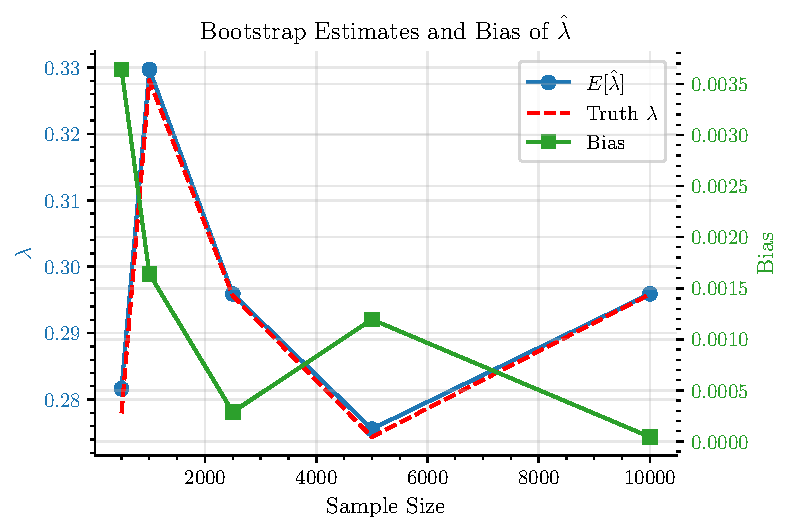
\includegraphics[width=0.51\textwidth]{./images/bootstrap_sizes_estimates_with_bias.pdf}
    }
    \hspace{0.0\textwidth}
    \subfigure[]{
        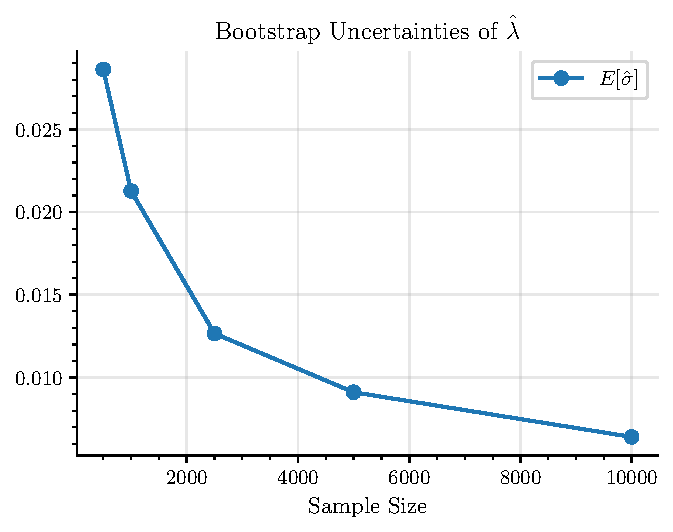
\includegraphics[width=0.43\textwidth]{./images/bootstrap_sizes_uncertainties.pdf}
    }
    \caption{(a) Bootstrap estimates of \(\hat{\lambda}\) as a function of sample size. The plot compares the mean bootstrap estimate \(E[\hat{\lambda}]\) (blue solid line with circles) with the true value of \(\lambda\) (red dashed line) and displays the corresponding bias (green solid line with squares). Bias decreases with increasing sample size. 
(b) Bootstrap uncertainties \(E[\hat{\sigma}]\) of \(\hat{\lambda}\) as a function of sample size, showing a steady decline in uncertainty as the sample size grows.}
    \label{fig:sample_sizes}
\end{figure}

\newpage
\section{sWeights Projecting and Fit}

In this case, our objective is to extract the properties of the signal in the $Y$ dimension using a one-dimensional fit. In this scenario, the background distribution in the $Y$ dimension, referred to as the control variable dimension, is unknown. To address this, we utilize sWeights to project onto this dimension.

Given the limited sample sizes, we employ an unbinned extended maximum likelihood estimation to first fit the data in the $X$ variable, which serves as the discriminant variable. 

Then, we use sWeights to extract the pure $h_s(Y)$ component. This is achieved through a weight function $w_s(X)$ such that:

Then, we use sWeights to project out pure $h_s(Y)$ component, which use a weight function $w_s(X)$ to make:

$$\int w_s(X)f(X,Y)=fh_s(Y).$$

This process has been implemented by \inlinecode{sweights} package \cite{DEMBINSKI2022167270}.

In a sample size of 10000, we present the weight functions for the signal and background, as well as the projected signal and background distributions in the $Y$ dimension. These results are depicted in Figure \ref{fig:weights_histograms}.

\begin{figure}[t]
    \centering
    \subfigure[]{
        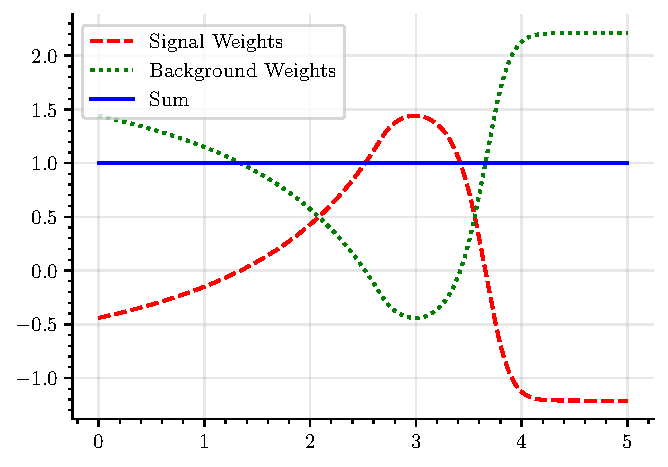
\includegraphics[width=0.5\textwidth]{./images/weights.pdf}
    }
    \hspace{0.0\textwidth}
    \subfigure[]{
        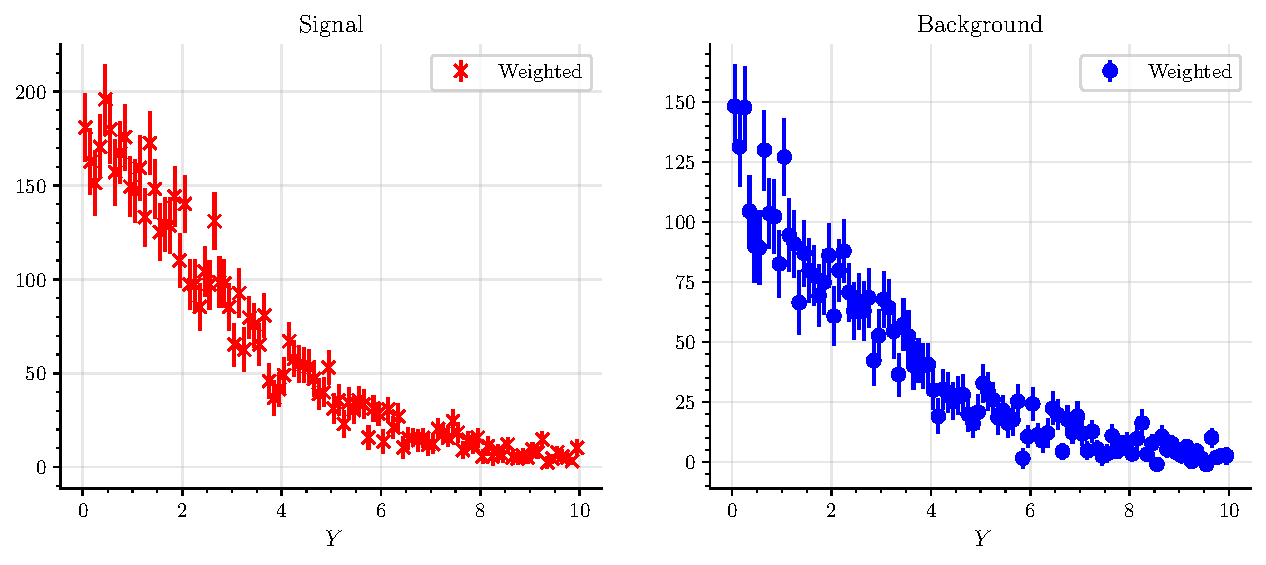
\includegraphics[width=0.93\textwidth]{./images/weighted_histograms.pdf}
    }
    \caption{(a) Signal and background weights.
(b) Projected distributions with error bars.}
    \label{fig:weights_histograms}
\end{figure}

By fitting these projected distributions, we can extract the desired signal properties in the $Y$ dimension.

\paragraph{Change Sample Sizes and Fit}

In \texttt{notebooks/f\_sWeights.ipynb}, we use the same samples as in Section \ref{sec:pbe}, stored in \texttt{notebooks/all\_samples.npy}.

We repeat the process of fitting in the $X$ dimension, calculating the weights, and projecting the data across different sample sizes. The results are summarized in Table \ref{tab:sw_sample_size_estimates}, where the "truth" value is $\lambda = 0.3$. For clarity, these results are also visualized in Figure \ref{fig:sw_sample_sizes}.

Compared to findings from the previous part, the value of $\hat{\lambda} - 
\lambda$ is not neglectable for all sample sizes, based on which we cannot determine the estimates are unbiased. Furthermore, The true bias can be estimated using bootstrapping, although this has not been implemented here.

On the other hand, even though slightly larger than the previous part, the estimated uncertainties steadily decreases with the sample sizes.


\begin{figure}[t]
    \centering
    \subfigure[]{
        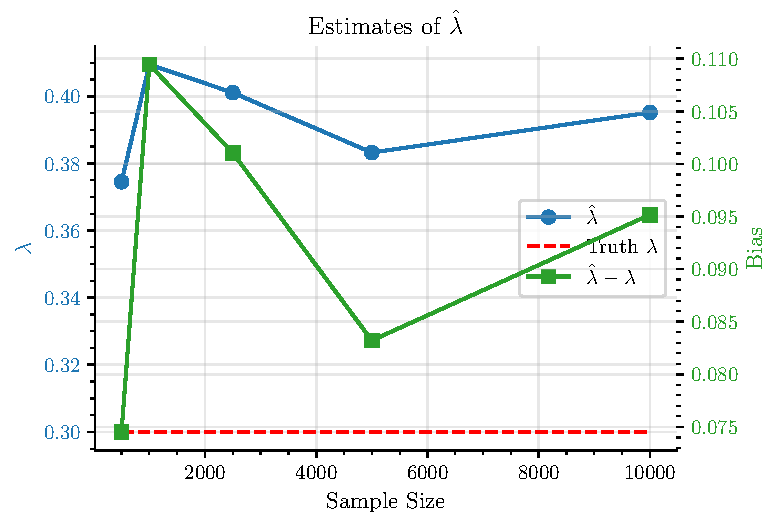
\includegraphics[width=0.51\textwidth]{./images/sweight_sizes_estimates.pdf}
    }
    \hspace{0.0\textwidth}
    \subfigure[]{
        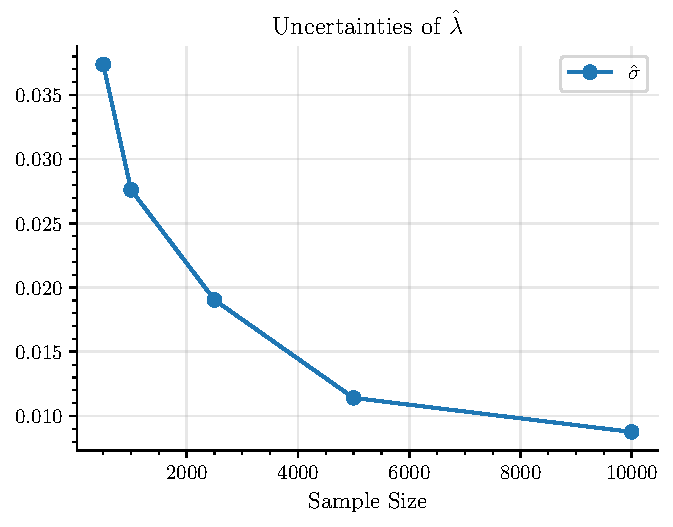
\includegraphics[width=0.43\textwidth]{./images/sweight_sizes_uncertainties.pdf}
    }
    \caption{(a) Estimates of $\hat{\lambda}$ for varying sample sizes.
(b) Corresponding uncertainties ($\hat{\sigma}$) as a function of sample size.}
    \label{fig:sw_sample_sizes}
\end{figure}


\begin{longtable}{llll}
\caption{Comparison of parameter estimates, uncertainties, and true values across sample sizes.}\label{tab:sw_sample_size_estimates}\\
\toprule
\textbf{Sample Size} & \textbf{$\hat{\lambda}$} & \textbf{$\hat{\sigma}$} & \textbf{Truth $\lambda$} \\
\midrule
\endfirsthead
\toprule
\textbf{Sample Size} & \textbf{$\hat{\lambda}$} & \textbf{$\hat{\sigma}$} & \textbf{Truth $\lambda$} \\
\midrule
\endhead
\bottomrule
\endfoot
500 & 0.374516 & 0.037371 & 0.3 \\
1000 & 0.409456 & 0.027608 & 0.3 \\
2500 & 0.401050 & 0.019033 & 0.3 \\
5000 & 0.383212 & 0.011413 & 0.3 \\
10000 & 0.395165 & 0.008759 & 0.3 \\
\end{longtable}


\section{Comparison of Two Methods}

\paragraph{Multi-Dimensional Likelihood Fit}

Theoretically, the multi-dimensional likelihood fit is more computationally expensive because the search space grows exponentially, and the likelihood surface can be more complex. Furthermore, it requires more apriori knowledge, such as the distribution in the dimensions of interest.

However, this computational cost comes with a trade-off: the method is more accurate in practice.

In scenarios where the distributions of components in the dimensions of interest are well understood and the search space is not excessively large, the multi-dimensional likelihood fit is both a straightforward and effective choice.



\paragraph{sWeights Projecting and One-Dimensional Fit}
One advantage of the sWeights method is its ability to handle situations where the properties in the control variable dimension are unknown. Theoretically, sWeights can perfectly extract the distribution in that dimension.

Moreover, because the method involves fitting only the projection in a single dimension, it is computationally more efficient. If the extraction is performed perfectly, it is as accurate as using same fit method in multi-dimension.

However, in this case, the extraction is not so perfect, and introduces errors in the estimate. 

In scenarios where the distributions of components in the dimensions of interest are not well understood, sWeights provides a crucial alternative.



\clearpage
\newpage
\appendix
\section{Use of AI Tools}
The following describes how AI tools were utilized in the preparation of this report:
\begin{itemize}
    \item \textbf{ChatGPT 4o}
        \begin{itemize}
            \item \textbf{Drafting} - Used for drafting certain sections of the report, including the frist section and Appendix. Also used for drafting captions of figures and tables.
            \item \textbf{Proofreading} - Reviewed grammatical correctness, improved sentence structure, and suggested alternative wordings for clarity across the report.
            \item \textbf{LaTeX Assistance} - Helped resolve issues encountered during the LaTeX formatting process, such as debugging compilation errors, optimizing figure placement, and improving overall document layout.
        \end{itemize}
\end{itemize}


\section{Template Information}
This report was formatted using the LaTeX template from the given Example Coursework (by Michal Dorko). Some modifications were made.

\newpage
\printbibliography
\end{document}